\index{Component!Names!Reassigning}
\index{Reassigning!Component Names}
\index{View!Component Names}
\index{Component!Names!View}
\index{Names!Component!Reassigning}
\index{Component!Names!Local}
\index{Component!Names!Global}
\index{Local Component Names}
\index{Global Component Names}
\index{Component}

\bxtipp{The following section deals with entering component names in the \gdcompnamesview{} when you have added \gdcases{} from the library. For information on component names in \gdsteps{}, see the \gdsteps{} section \bxpref{specsteps}.}

\begin{enumerate}
\item Once you have added a \gdcase{} from the library of \gdcases{} \bxpref{usingtemplate}, you will need to enter a component name for the component you want to test. 
\item In the \gdcompnamesview{}, you will see the \bxname{old name} for this component, which was given in the \gdstep{} contained in the library \gdcase{}. The old name is just a placeholder and should be \bxname{reassigned} (\bxfigref{compnamesview}).

\begin{figure}[h]
\begin{center}
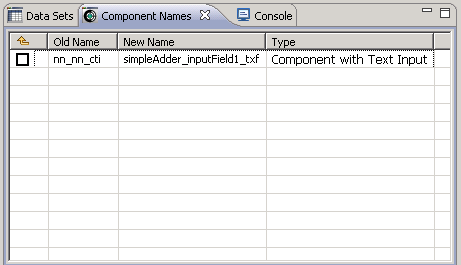
\includegraphics{Tasks/Compnames/PS/compnamesview}
\caption{The \gdcompnamesview{}}
\label{compnamesview}
\end{center}
\end{figure} 
 

\bxtipp{When you enter a component name in the \gdcompnamesview{}, you create a new reference to a component in the \gdaut{}. This component name appears in the \gdomeditor{} to be mapped to a component in your \gdaut{}. A \gdcase{} containing component names to be reassigned can therefore be used at a variety of different places to test different actual components. If you want to rename a component name, you can do so in the \gdcompnamebrowser{} \bxpref{TasksRenameCompName}.}

\item In the \bxname{new name} field, enter your name for this component, e.g. \bxshell{MainWindow\_NavigationTree\_tre}. 

We recommend using naming conventions for component names \bxpref{BPComponentNames}. 

\item Press \bxkey{Ctrl+SPACE} to see a list of component names you have already used for this type of component:

\begin{description}
\item[\bxname{Local}]{ component names are names you have used in this \gdcase{} for this component type. }
\gdmarpar{../../../share/PS/localName}{Local name}
\item [\bxname{Global}]{ component names are names you have used for this component type, but not in this \gdcase{}. }
\gdmarpar{../../../share/PS/globalName}{Global name}
%\item [Unused]{ component names are names that have already been mapped to this component type in the \gdaut{}. The \gdcase{} containing the component name has since been deleted.}
% \gdmarpar{../../../share/PS/OMLogName}{unused name}
 \end{description}

\item The component name you enter here will be collected by the \gdomeditor{} when you carry out object mapping so that you can assign it to a component in the \gdaut{}. 

\item Every time you want to carry out an action on this component, use this name. 
\end{enumerate}
\bxtipp{See the section on the component hierarchy for some tips on using component names in your tests \bxpref{TasksCompNameType}.}

\subsubsection{Writing \gdcases{} that can test different components in the \gdaut{}}
\gdhelpid{compNameViewContextId}{Component Names View}
\label{TasksCompNamesCheckbox}
Select the checkbox on the left of the \gdcompnamesview{} to be able to see and edit (reassign) this component name when you reuse the parent of the \gdcase{} you are editing. 

This is useful for creating flexible keywords that can be used for the same workflow on different components. Depending on what you want the keyword to do when you reuse it, you can reassign the name to test different components in the \gdaut{}.

\subsubsection{Changing component names}
If you newly reassign component names in  your test hierarchy that were themselves later reassigned, you will be shown a message in the \gdcompnamesview{}.
\begin{itemize}
\item The message only appears at places where you have reused the \gdcase{} containing that component, and where you have overwritten the component name. 
\item For example:
\begin{enumerate}
\item Your component was originally called \bxname{LoginDialog\_nn\_btn}.
\item You reused the \gdcase{} containing this component, and renamed the component \bxname{LoginDialog\_OK\_btn}.
\item You then change the component name in the original \gdcase{} to \bxcaption{LoginDialog\_AnyButton\_btn}.
\end{enumerate}
\item In the \gdcompnamesview{} for the reused \gdcase{}, you will see a warning message that the component name has no type.
\item You will also see the new name for the component.
\bxwarn{The warning field is not editable.}
\item If you want to keep the same overwritten name, enter the name into the \bxcaption{new name} field in the row for the new component name.
\item You can also change the overwritten name, or not overwrite it at all. In this case you will need to adapt your object mapping, if this component has been used in a \gdsuite{}. 
\item Once you have saved the \gdcompnamesview{}, the warning message will disappear. 
\end{itemize}
